
% LaTeX Beamer file automatically generated from DocOnce
% https://github.com/doconce/doconce

%-------------------- begin beamer-specific preamble ----------------------

\documentclass[handout]{beamer}

\usetheme{blue_shadow}
\usecolortheme{default}

% turn off the almost invisible, yet disturbing, navigation symbols:
\setbeamertemplate{navigation symbols}{}

% Examples on customization:
%\usecolortheme[named=RawSienna]{structure}
%\usetheme[height=7mm]{Rochester}
%\setbeamerfont{frametitle}{family=\rmfamily,shape=\itshape}
%\setbeamertemplate{items}[ball]
%\setbeamertemplate{blocks}[rounded][shadow=true]
%\useoutertheme{infolines}
%
%\usefonttheme{}
%\useinntertheme{}
%
%\setbeameroption{show notes}
%\setbeameroption{show notes on second screen=right}

% fine for B/W printing:
%\usecolortheme{seahorse}

\usepackage{pgf}
\usepackage{graphicx}
\usepackage{epsfig}
\usepackage{relsize}

\usepackage{fancybox}  % make sure fancybox is loaded before fancyvrb

\usepackage{fancyvrb}
\usepackage{minted} % requires pygments and latex -shell-escape filename
%\usepackage{anslistings}
%\usepackage{listingsutf8}

\usepackage{amsmath,amssymb,bm}
%\usepackage[latin1]{inputenc}
\usepackage[T1]{fontenc}
\usepackage[utf8]{inputenc}
\usepackage{colortbl}
\usepackage[english]{babel}
\usepackage{tikz}
\usepackage{framed}
% Use some nice templates
\beamertemplatetransparentcovereddynamic

% --- begin table of contents based on sections ---
% Delete this, if you do not want the table of contents to pop up at
% the beginning of each section:
% (Only section headings can enter the table of contents in Beamer
% slides generated from DocOnce source, while subsections are used
% for the title in ordinary slides.)
\AtBeginSection[]
{
  \begin{frame}<beamer>[plain]
  \frametitle{}
  %\frametitle{Outline}
  \tableofcontents[currentsection]
  \end{frame}
}
% --- end table of contents based on sections ---

% If you wish to uncover everything in a step-wise fashion, uncomment
% the following command:

%\beamerdefaultoverlayspecification{<+->}

\newcommand{\shortinlinecomment}[3]{\note{\textbf{#1}: #2}}
\newcommand{\longinlinecomment}[3]{\shortinlinecomment{#1}{#2}{#3}}

\definecolor{linkcolor}{rgb}{0,0,0.4}
\hypersetup{
    colorlinks=true,
    linkcolor=linkcolor,
    urlcolor=linkcolor,
    pdfmenubar=true,
    pdftoolbar=true,
    bookmarksdepth=3
    }
\setlength{\parskip}{7pt}  % {1em}

\newenvironment{doconceexercise}{}{}
\newcounter{doconceexercisecounter}
\newenvironment{doconce:movie}{}{}
\newcounter{doconce:movie:counter}

\newcommand{\subex}[1]{\noindent\textbf{#1}}  % for subexercises: a), b), etc

\usepackage{pgfpages} % for handouts

\logo{{\tiny Made with \href{https://github.com/doconce/doconce}{DocOnce}}}

%-------------------- end beamer-specific preamble ----------------------

% Add user's preamble




% insert custom LaTeX commands...

\raggedbottom
\makeindex

%-------------------- end preamble ----------------------

\begin{document}

% matching end for #ifdef PREAMBLE
% #endif

\newcommand{\exercisesection}[1]{\subsection*{#1}}

\input{newcommands_bfmath}
\input{newcommands_replace}


%\pgfpagesuselayout{4 on 1}[a4paper,landscape,border shrink=5mm]   % pdfnup is more flexible

% ------------------- main content ----------------------



% ----------------- title -------------------------

\title{Document for Testing Some Basic and Some Challenging Constructs in DocOnce Slides}

% ----------------- author(s) -------------------------

\author{Hans Petter Langtangen\inst{1,2}}
\institute{Simula Research Laboratory\inst{1}
\and
University of Oslo\inst{2}}
% ----------------- end author(s) -------------------------

\date{Jan 32, 2100
% <optional titlepage figure>
\ \\ 
{\tiny Made with \href{https://github.com/doconce/doconce}{DocOnce}}
}

\begin{frame}[plain,fragile]
\titlepage
\end{frame}

\section[First]{This is the first section}

\begin{frame}[plain,fragile]
\frametitle{Figure and bullet list}

\begin{columns}
\column{0.6\textwidth}
\pause
\begin{block}{Title with comma, and brackets: $[a,b]$ }
\footnotesize

\begin{itemize}
  \item Here is a \emph{wave signal} $f(x-ct)$

  \item It moves with velocity $c$

  \item But here it is just a figure
\end{itemize}

\noindent
\end{block}

\column{0.4\textwidth}
\begin{block}{}

\vspace{6mm}

% inline figure
\centerline{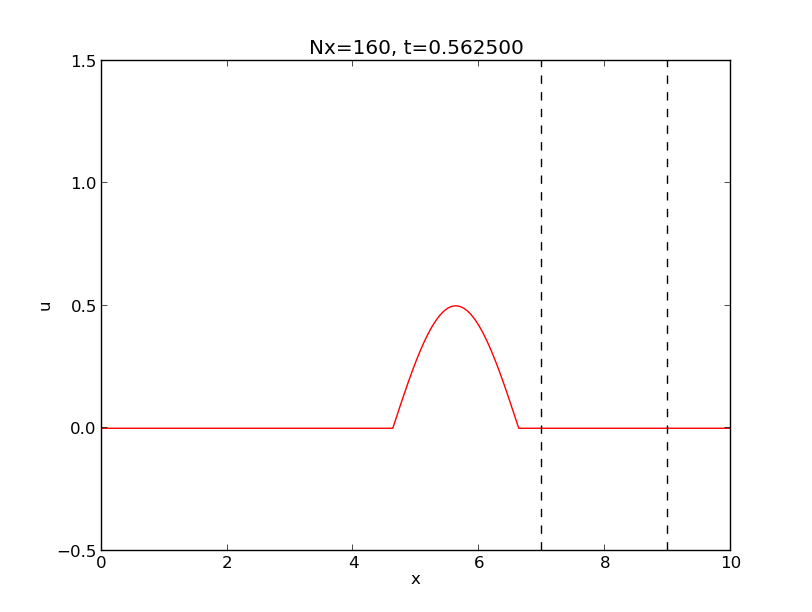
\includegraphics[width=0.7\linewidth]{testfigs/wave1D.png}}

\vspace{6mm}

\end{block}

\end{columns}
\end{frame}

\begin{frame}[plain,fragile]
\frametitle{Slide with pop-ups in red and notes}

\shortinlinecomment{hpl 1}{ Comments are typeset as usual in DocOnce. }{ Comments are typeset as }

\pause
Here we have a paragraph to pop up in red.\\
And a line more

\note{
One can also have ordinary notes.
Over multiple lines.
}
\end{frame}

\begin{frame}[plain,fragile]
\frametitle{A {\LaTeX} document}

\pause
\begin{minted}[fontsize=\fontsize{9pt}{9pt},linenos=false,mathescape,baselinestretch=1.0,fontfamily=tt,xleftmargin=2mm]{latex}
\documentclass[11pt]{article}
\usepackage{fancyvrb}
\begin{document}

\title{Here goes the title...}
\author{John Doe \and
Jane Doe\footnote{\texttt{jane.doe@cyber.net}.}}
\date{\today}
\maketitle

\end{minted}

\pause
\begin{block}{Notice}
{\LaTeX} has a lot of backslashes.
\end{block}

\pause
\begin{minted}[fontsize=\fontsize{9pt}{9pt},linenos=false,mathescape,baselinestretch=1.0,fontfamily=tt,xleftmargin=2mm]{latex}
\section{Heading}
bla-bla
\end{document}

\end{minted}
\end{frame}

\begin{frame}[plain,fragile]
\frametitle{An HTML document}

\begin{minted}[fontsize=\fontsize{9pt}{9pt},linenos=false,mathescape,baselinestretch=1.0,fontfamily=tt,xleftmargin=2mm]{html}
<html><head></head><body bgcolor="red">
<title>Here goes the title...<title>
<h1>Section heading</h1>
</body>
</html>

\end{minted}
\end{frame}

\section{Second section}

\begin{frame}[plain,fragile]
\frametitle{Second section}


\begin{block}{}

\vspace{6mm}

% inline figure
\centerline{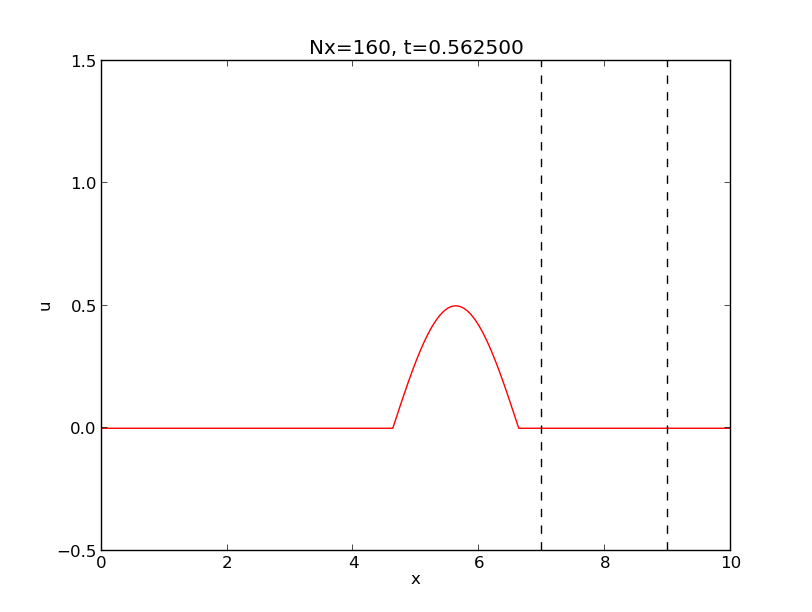
\includegraphics[width=0.8\linewidth]{testfigs/wave1D.png}}

\vspace{6mm}

\end{block}


\end{frame}

\begin{frame}[plain,fragile]
\frametitle{Some math and computer code}

\begin{block}{A simple, mathematical formula where $t\in [0,\pi]$: }
\[ f(x,y,t) = e^{-xt}\sin\pi y \]
\end{block}

\begin{block}{Bash demanded more of DocOnce than Python, so let's do Bash: }
First, inline \Verb@$? != 0@, then comments with dollar variables (and minted
style):







\begin{minted}[fontsize=\fontsize{9pt}{9pt},linenos=false,baselinestretch=1.0,fontfamily=tt,xleftmargin=2mm]{bash}
var=10
# $1, $2, ... are command-line args
if [ $? -eq 0 ]; then   # $? reflects success or not
  echo "Great!"
fi

\end{minted}

\end{block}
\end{frame}

\begin{frame}[plain,fragile]
\frametitle{Pop ups inside code blocks (for Beamer slides only)}

\begin{minted}[fontsize=\fontsize{9pt}{9pt},linenos=false,mathescape,baselinestretch=1.0,fontfamily=tt,xleftmargin=2mm]{python}
def f(x):
    return 42 + x

(*@\pause@*)
def g(x):
    return f(42)

(*@\pause@*)
print(g(13))

\end{minted}
\end{frame}

\begin{frame}[plain,fragile]
\frametitle{Various admon blocks}

Can use admons to simulate blocks:

\pause
\begin{block}{Key PDE (with large title and math font): }
\large

\[ \frac{\partial u}{\partial t} = \nabla^2 u \]
\end{block}

\pause
\begin{block}{}
Just some block with text and a conclusion that something is important.
This one pops up after the rest of the slide.
\end{block}

\pause
\begin{block}{Warning}
\footnotesize

Can use, e.g., a warning admon to have my own notes, preferably
inside preprocess/mako if statements to turn notes on and off.
This one is typeset in a small font and with the default
title (Warning) since no title is specified.
\end{block}
\end{frame}

\end{document}
